\documentclass{article}

\usepackage{amssymb}
\usepackage{float}
\usepackage[utf8]{inputenc}
\usepackage[english,ukrainian]{babel}
\usepackage{array}
\usepackage{graphicx}
\usepackage{mathtools}
\graphicspath{  {./images/} }
\setcounter{section}{-1}

\title{Розрахункова Робота 2 \\
        з математичної статистики\\ 
        Варіант 133}
\author{Воробйов Георгій}
\begin{document}

\maketitle

\tableofcontents

\section{Завдання}
\begin{enumerate}
    \item Проведiть первинний аналiз вибiрки. Це включає статистичний ряд (для розподiлiв —
        iнтервальний), емпiричну функцiю розподiлу (для неперервних розподiлiв iнтервальну), її
        графiк, полiгон частот (для дискретних розподiлiв), гiстограму (неперервнихрозподiлiв), box-and-whisker 
        plot.
    \item Знайдiть вибiркове середнє, вибiркову дисперсiю, виправлену вибiркову дисперсiю, вибiркову
        медiану, вибiркову моду, вибiрковi коефiцiєнти асиметрiї та ексцесу.
    \item Обґрунтуйтета висуньте (нову) гiпотезу про розподiл генеральної сукупностi. 
    \item Методом моментiв та методом максимальної вiрогiдностi знайдiть оцiнки параметрiв
        розподiлу. В деяких випадках це може бути не дуже просто (як, наприклад, для
        параметра N бiномiальної генеральної сукупностi). Це чудовий спосiб проявити креативнiсть
        та/або вмiння користуватися Google.
    \item Для кожного параметра кращу з цих двох оцiнок перевiрте на (асимптотичну)незмiщенiсть, консистентнiсть 
        та ефективнiсть.
    \item Побудуйте довiрчi iнтервали надiйнiстю0:95для параметрiв розподiлу.
    \item Нарештi, перевiрте висунуту гiпотезу про розподiл генеральної сукупностi за
        допомогою критерiю $\chi^2$
    \item Проявiть всi свої лiтературнi здiбностi та напишiть висновки
\end{enumerate}
Задана вибірка: \\ 
2  1  1  4  4  3  4  3  2  7  6  1  5  3  3  1  4  3  2  3  2  3  2  3  4 5  3  5  5  1  2  3  6  3
5  5  2  5  2  2  0  3  0  2  6  2  3  4  3  2 4  1  4  3  4  2  4  1  4  5  5  3  3  3  2  4  3  2
4  3  3  3  3  4  2 3  6  1  2  3  3  4  0  3  5  1  4  4  3  3  1  3  3  6  2  2  3  2  5  3 
\section{Розв'язок}
\subsection{Вступ}
Запишемо відсортовану вибірку: \\
0 0 0 1 1 1 1 1 1 1 1 1 1 2 2 2 2 2 2 2 2 2 2 2 2 2 2 2 2 2 2 2 2 3 3 3 3 3 3 3 3 3 3 3 3 3 3 3 3 3
3 3 3 3 3 3 3 3 3 3 3 3 3 3 3 3 4 4 4 4 4 4 4 4 4 4 4 4 4 4 4 4 4 5 5 5 5 5 5 5 5 5 5 5 6 6 6 6 6 7
\subsection{Аналіз вибірки}
Побудуємо статистичний ряд даної вибірки
\begin{center}
    \begin{tabular}{|c||m{2cm}|m{2cm}|m{2cm}|m{2cm}|}
        \hline
        елементи & Частота $n_i$ & Кумулятивна частота $n^*_i$ & Відносна частота $\nu_i$ & Відносна
        кумулятивна частота $\nu^*_i$ \\
        \hline \hline
        0 & 3  & 3   & 0.03 & 0.03 \\
        \hline
        1 & 10 & 13  & 0.1  & 0.13 \\
        \hline
        2 & 20 & 33  & 0.2  & 0.33 \\
        \hline
        3 & 33 & 66  & 0.33 & 0.66 \\
        \hline
        4 & 17 & 83  & 0.17 & 0.83 \\
        \hline
        5 & 11 & 94  & 0.11 & 0.94 \\
        \hline
        6 & 5  & 99  & 0.05 & 0.99 \\
        \hline
        7 & 1  & 100 & 1   & 1 \\
        \hline
    \end{tabular}
    
\end{center}
\newpage
За даними таблиці можемо побудувати полігон частот та функцію розподілу 
\begin{figure}[H]
    \centering
    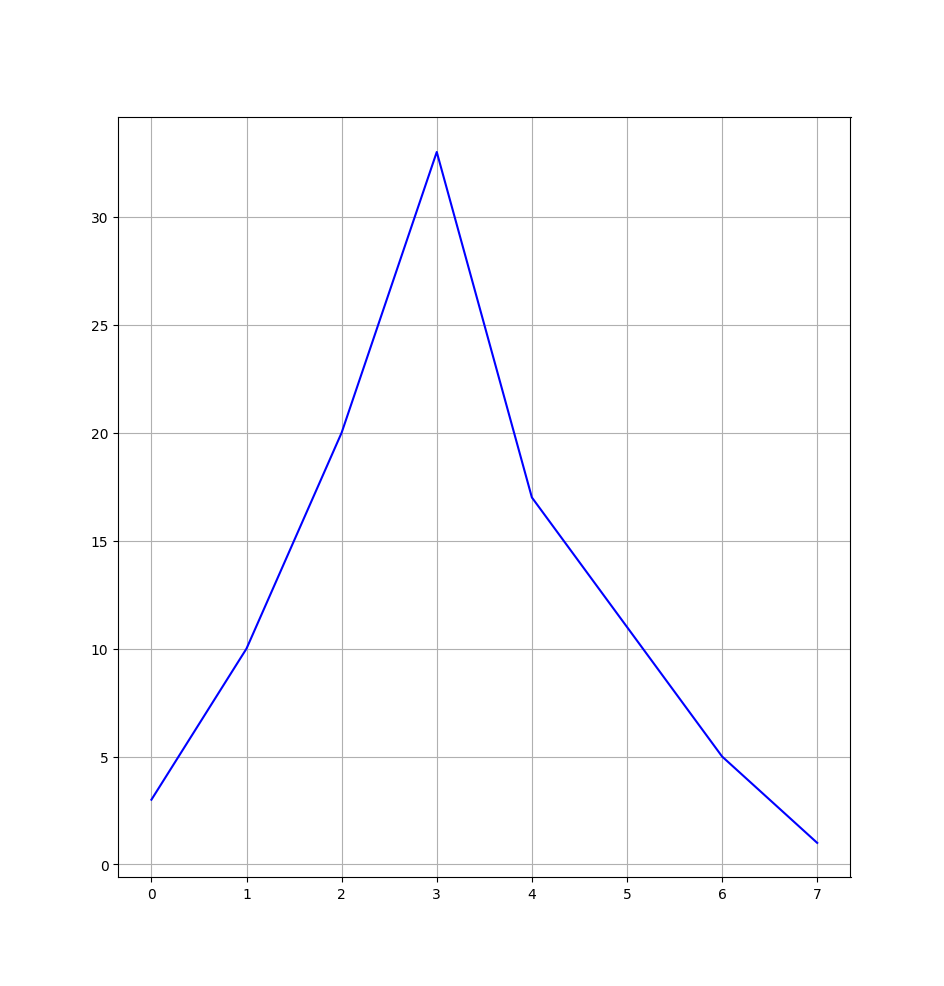
\includegraphics[width=\textwidth]{polygon.png} 
    \caption{Полігон частот}
\end{figure}
Маємо наступну емпіричну функцію розподілу
$$F^*_n(x) =
\begin{cases}
    0    & x \leq 0 \\
    0.03 & 0 < x \leq 1 \\
    0.13 & 1 < x \leq 2 \\
    0.33 & 2 < x \leq 3 \\
    0.66 & 3 < x \leq 4 \\
    0.83 & 4 < x \leq 5 \\
    0.94 & 5 < x \leq 6 \\
    0.99 & 6 < x \leq 7 \\
    1    & x > 7 \\
\end{cases}
    $$
Відповідний їй графік:
\begin{figure}[H]
    \centering
    \caption{Епірична функція розподілу}
    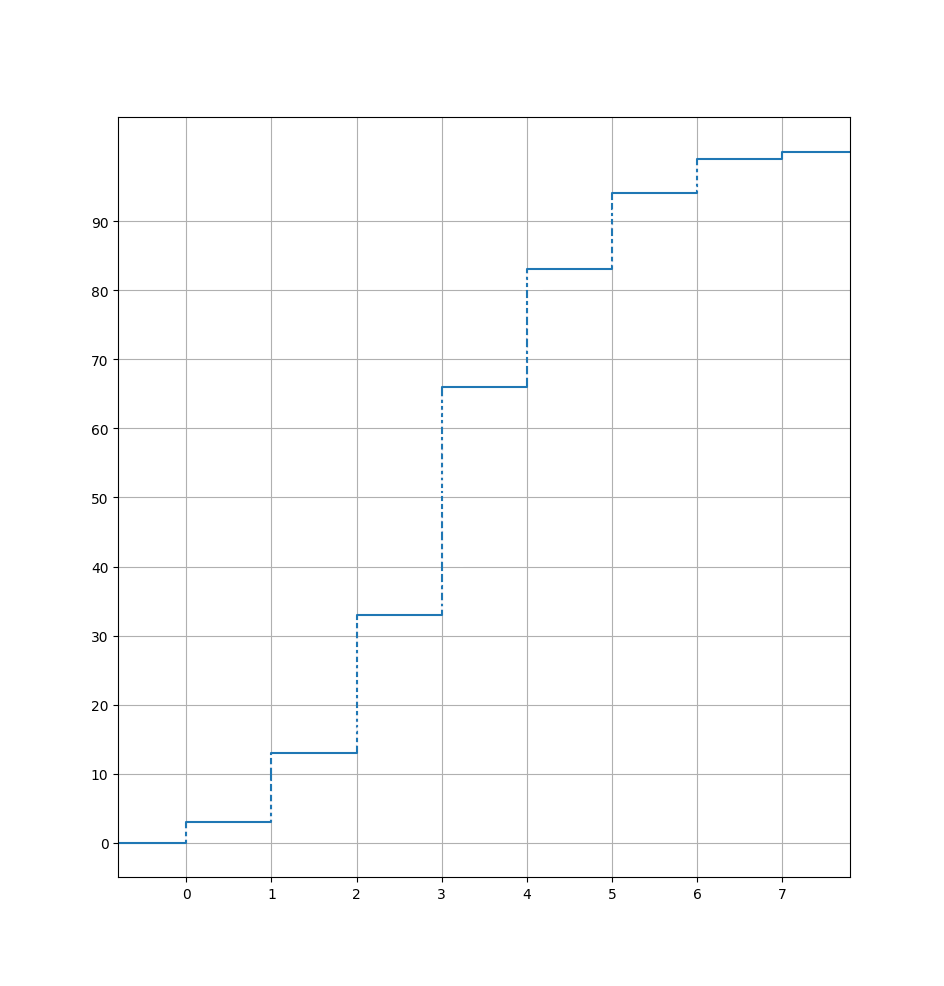
\includegraphics[width=0.8\textwidth]{empiric.png} 
\end{figure}
\begin{figure}[H]
    \centering
    \caption{Box and whisker plot}
    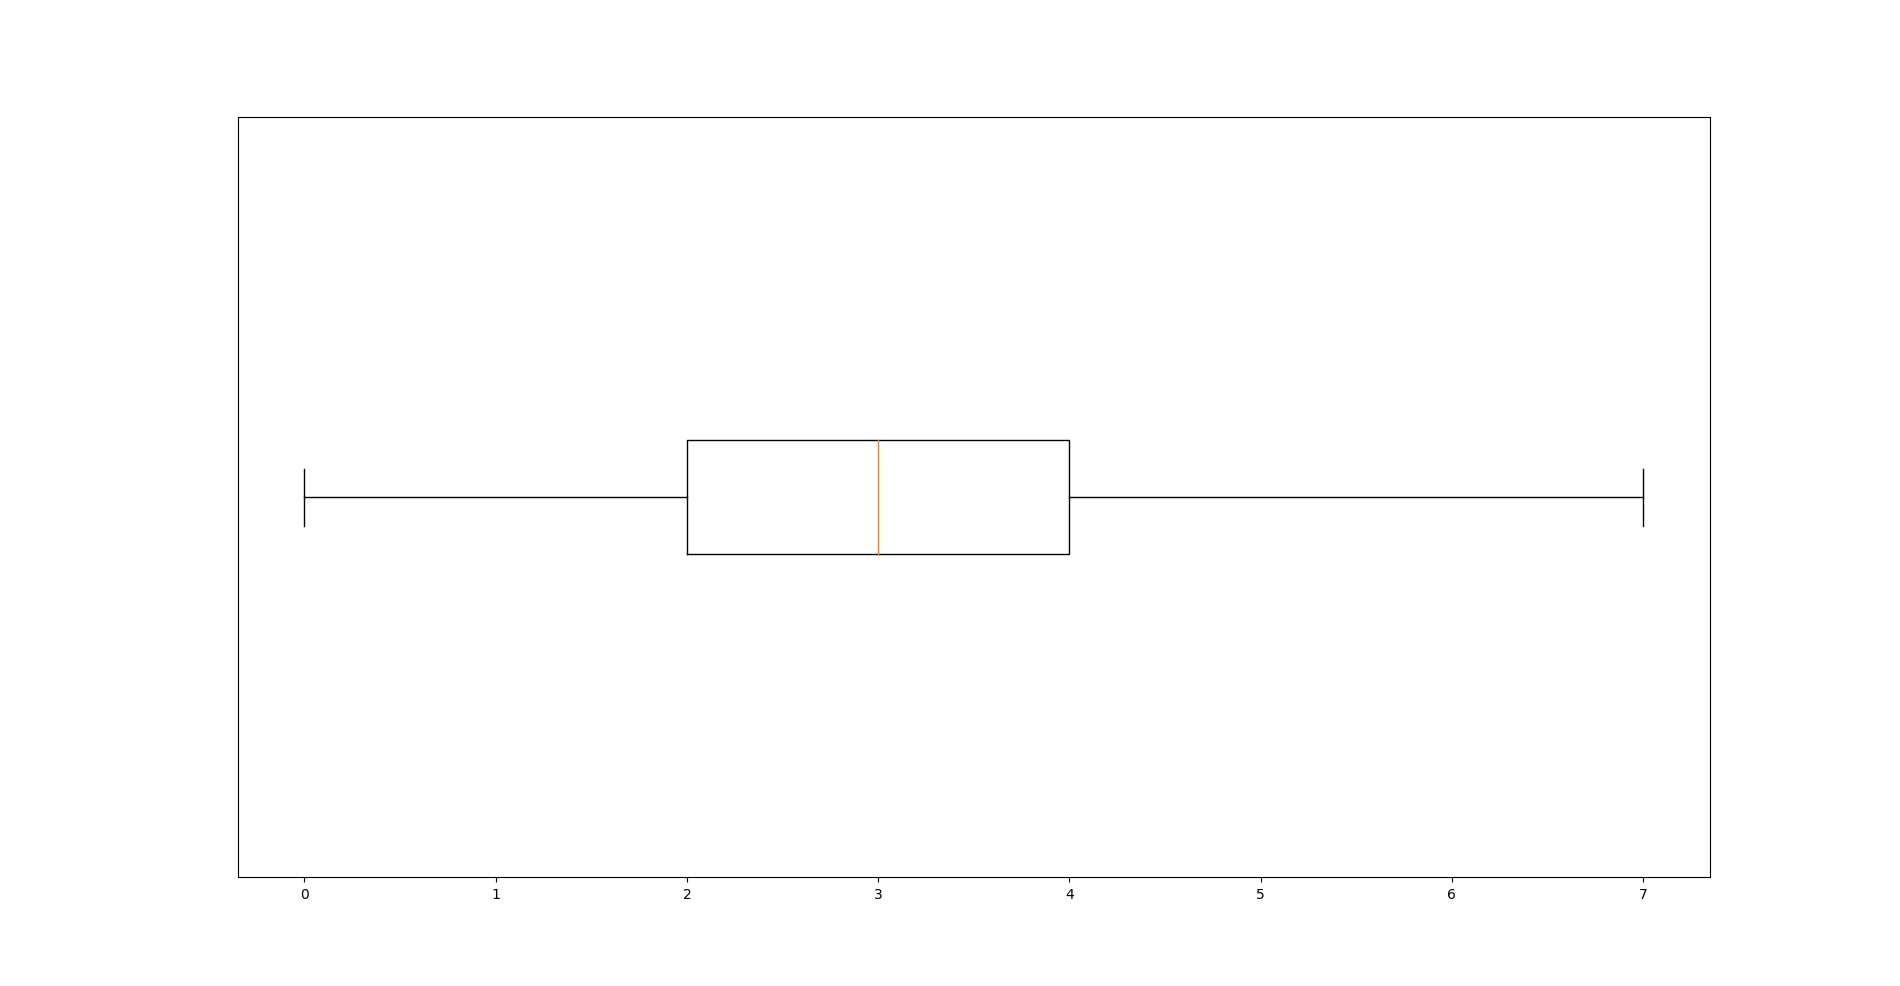
\includegraphics[width=\textwidth]{BandW.png} 
\end{figure}
\newpage
\section{Вибіркові статистики}
Порахуємо значення вибіркового середнього:
$$\overline{\xi}=\frac{1}{n}\sum_{i=1}^{100} \xi_i = 3.09$$
Порахуємо значення вибіркової дисперсії:
$$\mathbb{D}^{**}=\frac{1}{n} \sum_{i=1}^{100} (\xi_i - \overline{\xi})^2 = 2.08$$
Порахуємо значення виправленої вибіркової дисперсії:
$$\mathbb{D}^{***}=\frac{n}{n-1}\mathbb{D}^{**} = 2.06$$
Порахуємо вибіркову медіану:
$$Me^*\xi = \left<\text{cередина вибірки}\right> = 3$$
Порахуємо вибіркову моду - значення вибірки, що зустрічається найчастіше: 
$$Mo^*\xi = 3$$
Для розрахунку вибіркових коефіцієнтів асиметрії та ексцесу розрахуємо потрібні початкові та
центральні вибіркові моменти

$$As^* \xi = \frac{\mu_3^*}{({\sigma^*})^3}$$

$$Ex^* \xi = \frac{\mu_4^*}{({\sigma^*})^4} - 3$$

$$\mu_3^* = \mathbb{E}\left[ \xi - \overline{\xi}\right]^3 = 0.667$$

$$\mu_4^* = \mathbb{E}\left[ \xi - \overline{\xi}\right]^4 = 12.429$$

$$\sigma^* = \sqrt{\mathbb{D}^{**}} = 1.443$$

$$As^*\xi = 0.221$$

$$Ex^*\xi = -0.14$$

\newpage
\section{Висунення Гіпотези}
\begin{enumerate}
    \item Маємо дискретну ГС
    \item Значення дисперсії менше ніж математичного сподівання(Що схоже на npq та np відповідно)
\end{enumerate}
Тож можемо припустити, що данна ГС є розподіленою біноміально \\ $\xi \sim Bin(N, p)$
\section{Оцінки параметра розподілу}
\end{document}
